\documentclass{article}
\usepackage{amsmath} % For math equations
\usepackage{amsfonts} % For math fonts
\usepackage{amssymb} % For math symbols
\usepackage{float}
\usepackage{enumitem}
\usepackage{graphicx}
\setlist[enumerate,1]{label=\arabic*.}
\setlist[enumerate,2]{label=\alph*.,itemindent=2em}

\title{Homework 6}
\author{Asher Christian 006-150-286}
\date{2024-06-01}

\begin{document}
    \maketitle
    \section{Problem 1}
    Two discrete random variables $(X, Y ) \sim p(x, y) = P (X = x, Y = y), x \in \{1, 2\}, y \in \{1, 2, 3\}, p(1, 1) = .1, p(1, 2) = .1, p(1, 3) = .2, p(2, 1) = .1, p(2, 2) = .2, p(2, 3) = .3.$
    \begin{enumerate}
        \item Calculate $p(x) = P(X = x)$ and $p(y) = P (Y = y)$ for all possible $x$ and $y$.
            \[
            p(x) = \sum_{y}^{}p(x,y) = 
            \begin{cases}
                0.1 + 0.1 + 0.2 = 0.4 & x = 1\\
                0.1 + 0.2 + 0.3 = 0.6 & x = 2\\
            \end{cases}
            .\] 
            \[
            p(y) = \sum_{x}^{}p(x,y) = 
            \begin{cases}
                0.1 + 0.1 = 0.2 & y = 1\\
                0.1 + 0.2 = 0.3 & y = 2\\
                0.2 + 0.3 = 0.5 & y = 3\\
            \end{cases}
            .\] 
        \item Calculate $p(x|y) = P (X = x|Y = y)$ and $p(y|x) = P (Y = y|X = x)$ for all possible $x$ and $y$.
            \[
            p(x|y) = \frac{p(x,y)}{p_y(y)} = 
            \begin{cases}
                \frac{0.1}{0.2} = 0.5 & x=1,y=1\\
                \frac{0.1}{0.2} = 0.5 & x=2,y=1\\
                \frac{0.1}{0.3} = 0.\overline{3} & x=1, y=2\\
                \frac{0.2}{0.3} = 0.\overline{6} & x=2, y=2\\
                \frac{0.2}{0.5} = 0.4 & x=1, y=3\\
                \frac{0.3}{0.5} = 0.6 & x=2, y=3\\
            \end{cases}
            .\] 
            \[
            p(y|x) = \frac{p(x,y)}{p_x(x)} =
            \begin{cases}
                \frac{0.1}{0.4} = 0.25 & y=1, x=1\\
                \frac{0.1}{0.4} = 0.25 & y=2, x=1\\
                \frac{0.2}{0.4} = 0.50 & y=3, x=1\\
                \frac{0.1}{0.6} = 0.1\overline{6} & y=1, x=2\\
                \frac{0.2}{0.6} = 0.\overline{33} & y=2, x=2\\
                \frac{0.3}{0.6} = 0.50 & y=3,x=3\\
            \end{cases}
            .\] 
        \item Calculate $E(X,Y ), E(X), E(Y )$, and $Cov(X, Y )$.
            \[
            E(XY) = \sum_{x}^{}\sum_{y}^{}xyp(x,y) = 1*0.1 + 2*0.1 + 3*0.2 + 2*0.1+ 4*0.2 + 6*0.3 = 3.7
            .\] 
            \[
            E(X) = \sum_{x}^{}xp_x(x) = 1*0.4 + 2*0.6 = 1.6
            .\] 
            \[
            E(Y) + \sum_{y}^{}yp_y(y) = 1*0.2 + 2*0.3 + 3*0.5 = 2.3
            .\] 
            \[
            Cov(X,Y) = E((X-E(X))(Y-E(Y)) = \sum_{x}^{}\sum_{y}^{}(X-E(X))(Y-E(Y))p(x,y)
            .\] 
            $= (1-1.6)(1-2.3)(0.1) + (1-1.6)(2-2.3)(0.1) + (1-1.6)(3-2.3)(0.2) + (2-1.6)(1-2.3)(0.1) + (2-1.6)(2-2.3)(0.2) + (2-1.6)(3-2.3)(0.3) = 0.02$

    \end{enumerate}
    \section{Problem 2}
    Suppose we observe $(X_i, Y_i) \sim f (x, y)$ independently for $i = 1, ..., n.$ Let $\bar{X} =\sum_{i=1}^{n} \frac{X_i}{n}$, and $\bar{Y} = \sum_{i=1}^{n} \frac{Y_i}{n}$. Let $\overline{X_i} = X_i - \bar{X}$, and $\overline{Y_i} = Y_i - \bar{Y}$. Let \textbf{X} be the vector formed by $( \overline{X_i}, i = 1, ..., n)$, and \textbf{Y} be the vector formed by $( \overline{Y_i}, i = 1, ..., n)$. For the following scatterplots of $(X_i, Y_i), i = 1, ..., n$, where each $(X_i, Y_i)$ is a point,
    \begin{enumerate}
        \item Write down the possible value of correlation for each scatterplot. You do not need to be precise.\\
            going left to right, 1, 0.8, 0.5, -0.5, -0.8, -1
        \item  Plot the vectors of \textbf{X} and \textbf{Y} for each scatterplot.

    \end{enumerate}
    \begin{figure}[H]
        \centering
        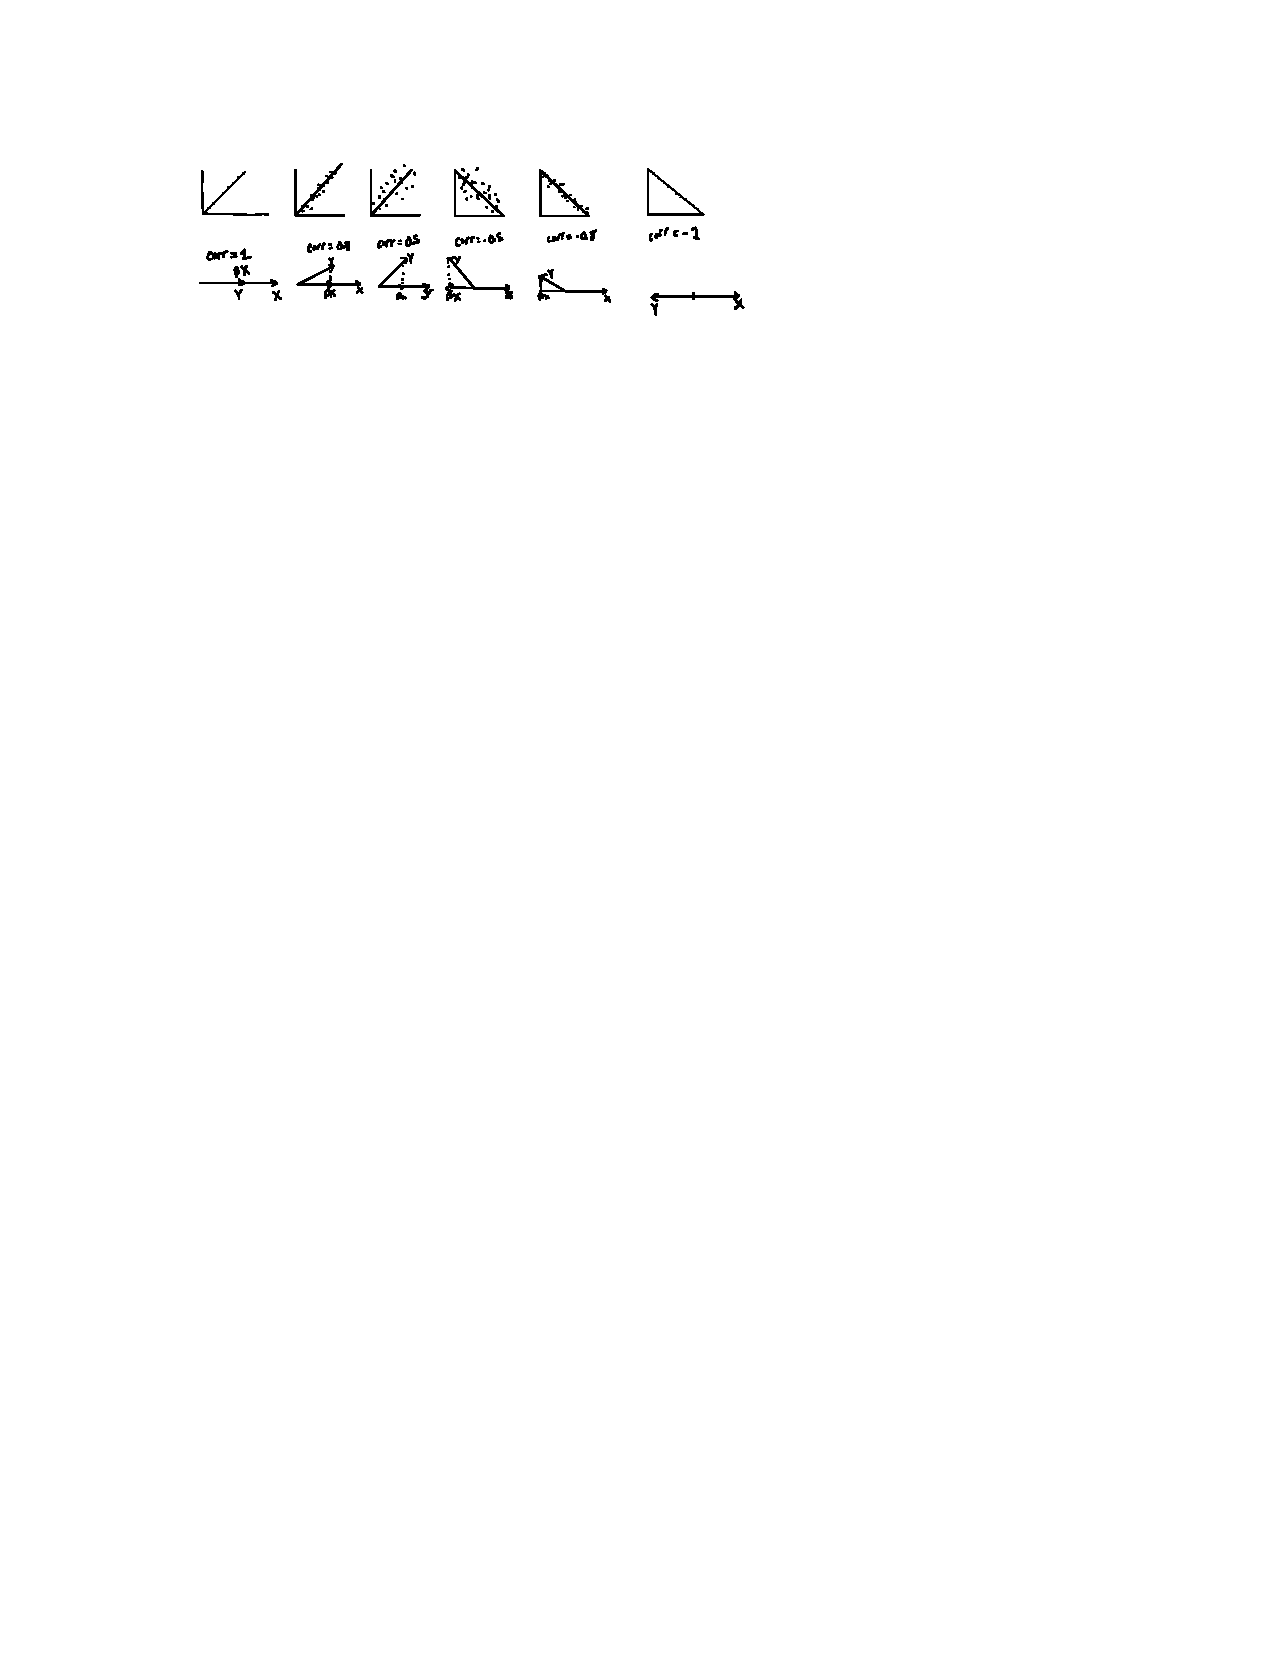
\includegraphics[width=\textwidth]{Problem_2.pdf}
        \caption{problem 2}
        \label{fig:my_image}
    \end{figure}

    \section{Problem 3}
    Assume $X \sim N(0,1),$ and $[X|X=x] \sim N(\rho x, 1-\rho^2).$
    \begin{enumerate}
        \item What are $f_X(x), f(y|x),$ and $f(x,y)$?
            \[
            f_X(x) = \frac{1}{\sqrt{2\pi }}e^{-\frac{x^2}{2}}
            .\] 
            \[
            f(y|x) = \frac{1}{\sqrt{2\pi (1-\rho^2)}}e^{-\frac{(y-\rho x)^2}{2(1-\rho^2)}}
            .\] 
            \begin{align*}
                f(x,y) &= f_X(x)f(y|x)\\ 
                       &= \frac{1}{2\pi \sqrt{1-\rho ^2}}\text{exp}(-\frac{x^2}{2}-\frac{(y-\rho x)^2}{2(1-\rho^2)})\\
                       &= \frac{1}{2\pi \sqrt{1-\rho ^2}}\text{exp}(-\frac{x^2(1-\rho ^2)+(y-\rho x)^2}{2(1-\rho ^2)})\\
                       &= \frac{1}{2\pi \sqrt{1-\rho ^2}}\text{exp}(-\frac{x^2+y^2-x^2\rho ^2-2\rho xy+\rho ^2x^2}{2(1-\rho ^2)})\\
                       &= \frac{1}{2\pi \sqrt{1-\rho ^2}}\text{exp}(-\frac{x^2+y^2-2\rho xy}{2(1-\rho ^2)})
            \end{align*}
        \item What are $E[Y|X = x]$ and $Var[Y|X = x]$?
            \begin{align*}
                E[Y|X=x] &= \int_{-\infty}^{\infty}f(Y|x)dy\\
                         &= \int_{-\infty}^{\infty}\frac{1}{2\pi (1-\rho ^2)}e^{-\frac{(y-\rho x)^2}{2(1-\rho ^2}}\\
                         &= E(\sqrt{(1-\rho ^2)}z+\rho x)\\
                         &= \rho x\\
                Var[Y|X=x] &= Var(\sqrt{(1-\rho^2)}z+\rho x)\\
                           &= (1-\rho^2 )
            \end{align*}
        \item Explain that we can express the model as $Y = \rho X + \epsilon $, where $\epsilon \sim N(0,1-\rho ^2)$, and $\epsilon $ is independent of $X$.\\
            We can express the model as this way because it is a reversion towards 0 of $\rho X$ and then an added variance to keep the overall variation
            of the population within the normal range of [0,1] and keeping the Y in the same distribution as the X because otherwise Y would converge to smaller
            and smaller variances.
        \item Based on (3), show that $E(Y) = 0, Var(Y) = 1, Cov(X,Y) = \rho $
            \[
            E(Y) = E(\rho X + \epsilon ) = \rho E(X) + E(\epsilon ) = 0
            .\] 
            \[
            Var(Y) = Var(\rho X + \epsilon ) = \rho ^2Var(X) + Var(\epsilon ) = \rho ^2+1-\rho ^2 = 1
            .\] 
            \begin{align*}
                Cov(X,Y) &= E((X-E(X))(Y-E(Y)))\\
                         &= E(XY)\\ 
                         &= \int_{-\infty}^{\infty}\int_{-\infty}^{\infty}xy \frac{1}{2\pi \sqrt{1-\rho ^2}}\text{exp}(-\frac{x^2+y^2-2\rho xy}{2(1-\rho ^2)})dxdy\\
                         &= E(X(\rho X+\epsilon )) \\
                         &= \rho E(X^2) + E(X\epsilon )\\
                         &= \rho * 1 + E(X)E(\epsilon )\\
                         &= \rho 
            \end{align*}
    \end{enumerate}
    \section{Problem 4}
    If two continuous random variables $X$ and $Y$ are independent, prove
    \begin{enumerate}
        \item $Cov(X,Y) = 0$. Please explain the reverse may not be true, i.e it is possible $Cov(X,Y) = 0$ even if $X$ and $Y$ are not independent.
            \begin{align*}
                Cov(X,Y) &= E[(X-E(X))(Y-E(Y))]\\
                         &= \int_{}^{}\int_{}^{}(X-E(X))(Y-E(Y))f(x,y)dxdy\\
                         &= \int_{}^{}\int_{}^{}(X-E(X))(Y-E(Y))f(x)f(y)dxdy\\
                         &= \int_{}^{}(X-E(X))f(x)dx\int_{}^{}(Y-E(Y))f(y)dy\\
                         &= E(X-E(X))E(Y-E(Y))\\
                         &= 0
            \end{align*}
            The inverse is not true because of non-linear relationships. If Y is related to
            X by a polynomial of degree greater than one, for example, the covariance may still be 0
            even when a true relationship exists.
        \item $Var(X+Y) = Var(X) + Var(Y)$
            \begin{align*}
                Var(X+Y) &= E[((X+Y)-E(X+Y))^2]\\
                         &- E[((X-E(X)) + (Y-E(Y)))^2]\\
                         &= E[(X-E(X))^2 + (Y-E(Y))^2 + 2(X-E(X))(Y-E(Y))]\\
                         &= Var(X) + Var(Y) +2Cov(X,Y)\\
                         &= Var(X) + Var(Y)
            \end{align*}
        \item If $X_1...,X_i...,X_n$ are independent and indentically distributed, with $E(X_i) = \mu $ and $Var(X_i) = \sigma ^2$. Let $\overline{X}$ be the average of $X_i, i=1,...,n$. Calculate $E(\overline{X})$ and $Var(\overline{X})$
            \begin{align*}
                E(\overline{X}) &= E(\frac{1}{n}\sum_{}^{}X_i)\\
                                &=\frac{1}{n} \sum_{}^{}E(X_i)\\
                                &= \frac{1}{n} n\mu \\
                                &= \mu \\
                Var(\overline{X}) &= Var(\frac{1}{n}\sum_{}^{}X_i)\\
                                  &= \frac{1}{n^2}\sum_{}^{}Var(X_i) \\
                                  &= \frac{1}{n^2} n \sigma ^2  \\
                                  &= \frac{\sigma ^2}{n}
            \end{align*}
    \end{enumerate}

\end{document}
